\documentclass[a4paper,ngerman,12pt]{scrartcl}

\usepackage[utf8]{inputenc}
%\usepackage[ansinew]{inputenc}

\usepackage[ngerman]{babel}

\usepackage{amsmath,amsthm,amssymb,stmaryrd,color,graphicx}
\usepackage{setspace}
\usepackage{bussproofs}
\usepackage{array}
\usepackage{comment}
\usepackage{wrapfig}

\usepackage{enumitem}

\usepackage{units}

\usepackage[protrusion=true,expansion=true]{microtype}

\usepackage{lmodern}

\usepackage{hyperref}
\usepackage{cleveref}

\newcommand{\RR}{\mathbb{R}}
\newcommand{\CC}{\mathbb{C}}
\newcommand{\ZZ}{\mathbb{Z}}
\newcommand{\NN}{\mathbb{N}}
\newcommand{\QQ}{\mathbb{Q}}

\setlength\parskip{\medskipamount}
\setlength\parindent{0pt}

\theoremstyle{definition}
\newtheorem{defn}{Definition}[]
\newtheorem{axiom}[defn]{Axiom}
\newtheorem{bsp}[defn]{Beispiel}

\theoremstyle{plain}
\newtheorem{prop}[defn]{Proposition}
\newtheorem{motto}[defn]{Motto}
\newtheorem{wunder}[defn]{Wunder}
\newtheorem{ueberlegung}[defn]{Überlegung}
\newtheorem{lemma}[defn]{Lemma}
\newtheorem{kor}[defn]{Korollar}
\newtheorem{hilfsaussage}[defn]{Hilfsaussage}
\newtheorem{satz}[defn]{Satz}
\newtheorem{frage}[defn]{Frage}

\theoremstyle{remark}
\newtheorem{bem}[defn]{Bemerkung}
\newtheorem{aufg}[defn]{Aufgabe}

\newtheorem*{antwort}{Antwort}

\newlength{\aufgabenskip}
\setlength{\aufgabenskip}{1.4em}
\newcounter{aufgabennummer}
\newenvironment{aufgabe}[1]{
	\addtocounter{aufgabennummer}{1}
	\textbf{Aufgabe \theaufgabennummer.} \emph{#1} \par
}{\vspace{\aufgabenskip}}

\clubpenalty=10000
\widowpenalty=10000
\displaywidowpenalty=10000

\setlength\unitlength{1cm}

\usepackage{tikz}

\RequirePackage{geometry}
\geometry{textwidth=16.0cm,textheight=24.5cm,footskip=1.5cm}

\begin{document}
	
\begin{picture}(0,0)
\put(0,-0.5){%
	
\includegraphics[scale=0.1]{logo-ifm}
}
\put(14.0,-3.5){%
	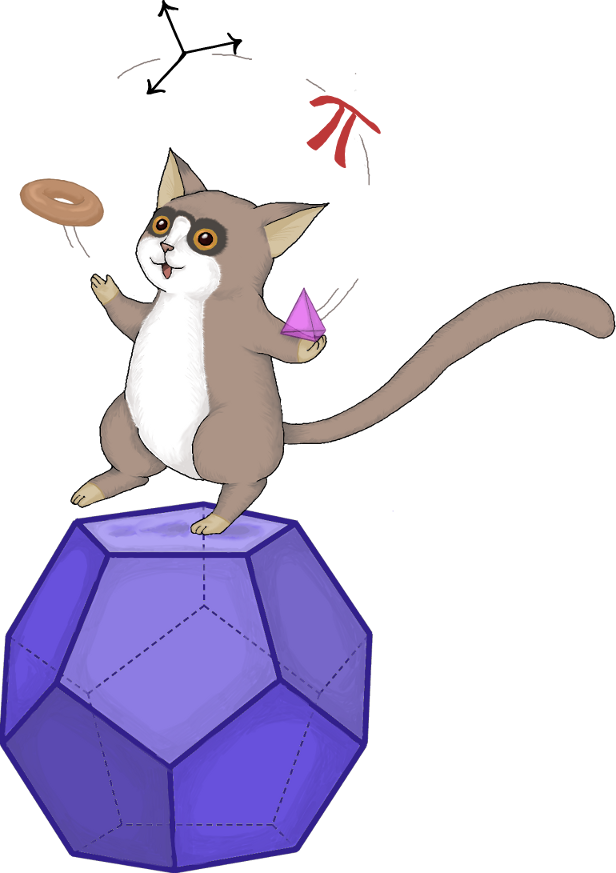
\includegraphics[scale=0.17]{cover}
}
\end{picture} 
	
\vspace{6em}

\section*{Unmöglichkeitsbeweise über Invarianten - Lösungshinweise}

Dieses Skript enthält Lösungs\emph{hinweise} zum letzten Korrespondenzbrief. Manchmal sind dies schon die kompletten Lösungen der Aufgaben, meistens sind es aber nur einige Hinweise, die dir dabei helfen sollen, auch die Aufgaben lösen zu können, bei denen du bisher nicht weiter gekommen bist. Wenn du noch weitere Fragen zu den Aufgaben hast, kannst du uns diese weiterhin gerne per E-Mail stellen.

Wenn du uns bereits deine eigenen Lösungsversuche geschickt hast (oder noch schicken wirst - das ist selbstverständlich immer noch möglich), dann versuchen wir natürlich auch dir mit unseren Korrekturen beim Verständnis der Aufgaben zu helfen. Es lohnt sich also uns deine Lösungen zu senden :-)

\begin{aufgabe}{}
	\begin{enumerate}
		\item möglich (trivial)
		\item nicht möglich, da nur 62 Felder - nicht durch 4 teilbar
		\item nicht möglich, Beweis über zweites buntes Schachbrett (jedes Quadrat überdeckt ein Feld jeder Farbe - hier zwei schwarze und zwei grüne herausgeschnitten)
		\item möglich (\glqq trivial\grqq)
	\end{enumerate}
\end{aufgabe}

\begin{aufgabe}{}
	\begin{enumerate}
		\item möglich (trivial)
		\item nicht möglich, da nur 62 Felder - nicht durch 4 teilbar
		\item möglich (\glqq trivial\grqq)
		\item nicht möglich, Beweis über erstes buntes Schachbrett (jeder lange Stein überdeckt ein Feld jeder Farbe - hier zwei gelbe herausgeschnitten)
	\end{enumerate}
\end{aufgabe}

\begin{aufgabe}{Dreieckstetrominos}
	Nicht möglich mit gleicher Begründung wie Tetromino-Fall:
	\begin{center}
		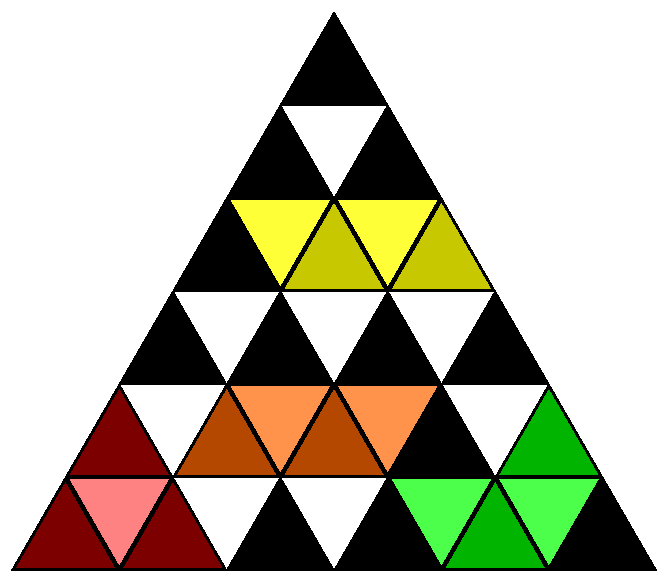
\includegraphics[width=.4\textwidth]{Bilder/Dreiecksschachbrett-Lsg.pdf}
	\end{center}
\end{aufgabe}

\begin{aufgabe}{}
	Möglich z.B. mit 4 gelben, 4 blauen und 1 grünen (nach einer Begegnung gelb+blau) - \textbf{beachte:} Hier ist $C = 4 - 1 = 3$ durch 3 teilbar!
	
	Nicht möglich für alle Startsituationen, in denen $C$ nicht durch $3$ teilbar (aber auch andere Startsituationen denkbar!).
\end{aufgabe}

\begin{aufgabe}{Chamäleonmünzen}
	Nicht möglich bei zwei Umdrehen (Anzahl der Bildmünzen immer durch $2$ teilbar (Beweis!) - aber für gleiches Verhältnis müssten 3 Bildmünzen da sein)
	
	Möglich für drei Umdrehen ()
\end{aufgabe}

\begin{aufgabe}{}
	\begin{enumerate}
		\item pro Spielzug genau zwei Münzen umdrehen musst? Unmöglich (wie oben)
		\item pro Spielzug genau drei Münzen umdrehen musst? Unmöglich (immer durch 3 teilbar!)
		\item pro Spielzug genau vier Münzen umdrehen musst? Unmöglich (wie oben)
	\end{enumerate}
\end{aufgabe}

\begin{aufgabe}{}
Beides unmöglich: Summe aller Zahlen bleibt immer gleich. Ist zu Beginn $1+2+3+4+5+6+7+8=36$ und das lässt sich nicht gleichmässig auf $8$ Zahlen verteilen.
\end{aufgabe}

\begin{aufgabe}{Produkte und Summen auf dem Schachbrett}
	Unmöglich, siehe \url{http://lwmb.de/pdf/lsg041.pdf} (Zweite Lsg!)
\end{aufgabe}

\end{document}